\section{4点関数\label{sec:fourpointfunc}}

この節では強結合領域$\beta J \gg 1$における4点関数を論じる。
disorder-averageを取る事によって最も一般的な4点関数は
\begin{align}
	\average{\psi_i(t_1)\psi_i(t_2)\psi_j(t_3)\psi_j(t_4)}
\end{align}
という形に制限される。
これを$i$と$j$について平均を取ったものを考える:
\begin{align}
	\frac{1}{N^2}\sum_{i,j=1}^{N}\average{T\psi_i(t_1)\psi_i(t_2)\psi_j(t_3)\psi_j(t_4)}
	= G(t_{12})G(t_{34}) + \frac{1}{N}\mathcal{F}(t_1, \cdots, t_4).
	\label{eq:fourpointfunc}
\end{align}
以下では$\mathcal{F}$について解析する。

\begin{figure}[h]
	\centering
	\vspace{1cm}
	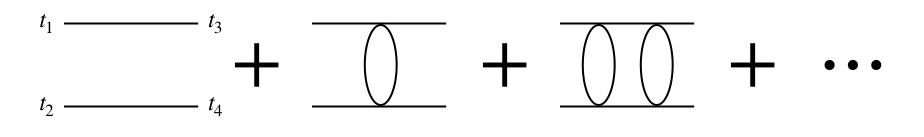
\includegraphics[width=13cm]{figures/ladderDiagram}
	\caption{\eqref{eq:fourpointfunc}式の$1/N$の項を表すダイアグラム。
		特に$q=4$の場合について描画した。ラダーダイアグラムと呼ぶ。}
	\label{fig:ladderdiagram}
\end{figure}

$\mathcal{F}$を表すダイアグラムはラダーダイアグラムである(図\ref{fig:ladderdiagram})。
$n$個の輪があるものを$\mathcal{F}_n$とすると、計算するべきは
\begin{align}
	\mathcal{F} = \sum_n \mathcal{F}_n
\end{align}
である。
図\ref{fig:ladderdiagram}の最初にある輪を持たないラダーダイアグラムは単なるプロパゲーターの積である:
\begin{align}
	\mathcal{F}_0(t_1, \cdots, t_4) = -G(t_{13})G(t_{24}) + G(t_{14})G(t_{23}).
\end{align}
次に並ぶ、輪を1個だけ持つラダーダイアグラムでは、輪の端の位置について積分した形で与えられる:
\begin{align}
	\mathcal{F}_1(t_1, &\cdots, t_4)\nonumber\\
	&= J^2(q - 1)\int dtdt'\ \left(
		G(t_1 - t)G(t_2 - t')G(t - t')^{q-2}G(t - t_3)G(t' - t_4) - (t_3 \leftrightarrow t_4)
	\right).
\end{align}
積分の前にある$q-1$という因子は、どの線をレールや輪にするかのパターン数に起因する。
上述した2つのラダーダイアグラム$\mathcal{F}_0$、$\mathcal{F}_1$に限らず、
全てのラダーダイアグラムは$1/N$に比例する。

あるラダーダイアグラム$\mathcal{F}_n$と次の$\mathcal{F}_{n+1}$の間には
\begin{align}
	\mathcal{F}_{n+1}(t_1, \cdots, t_4)
	= \int dtdt'\ K(t_1, t_2; t, t')\mathcal{F}_n(t, t', t_3, t_4)
	\label{eq:F_n+1_and_F_n}
\end{align}
という漸化式的な関係がある。
ここで積分核$K$は
\begin{align}
	K(t_1, t_2; t_3, t_4) = -J^2(q-1)G(t_{13})G(t_{24})G(t_{34})^{q-2}
	\label{eq:def_of_K}
\end{align}
である。
\eqref{eq:F_n+1_and_F_n}式の計算では、$K$の最初の2つの変数を1つめの添字、残りの2つを2つ目の添字
と見なす事によって積分を行列計算としてしまうのが便利である(行列$K$は2変数反対称関数の空間に作用する)。
こうする事で全てのラダーダイアグラムの総和を
\begin{align}
	\mathcal{F}
	= \sum_{n=0}^{\infty}\mathcal{F}_n
	= \sum_{n=0}^{\infty}K^n \mathcal{F}_0
	= \frac{1}{1 - K}\mathcal{F}_0
	\label{eq:geometric_series_of_F}
\end{align}
という様に表す事ができる。
これを更に計算するために、以下では$K$を対角化する事を考える。
\eqref{eq:def_of_K}式による定義では$K$は対称行列ではないが、
次のような操作により対称化する事が可能である:
\begin{align}
	\tilde{K}(t_1, t_2; t_3, t_4) \equiv
	|G(t_{12})|^{\frac{q-2}{2}}K(t_1, t_2; t_3, t_4)|G(t_{34})|^{\frac{2-q}{2}}.
	\label{eq:symmetric_K}
\end{align}
従って$K$は固有関数(固有ベクトル)の完全系を持つとして良い。

\subsection{$K_c$の対角化}
ここまでの話は一般の$\beta J$について成り立つ。
解析を進めるために、以下では共形対称性の成り立つ極限$\beta J \gg 1$で考える。
よって2点関数は$\eqref{eq:conformal_ansatz}$式の$G_c(t)$で与えられる。
\eqref{eq:conformal_ansatz}式を\eqref{eq:def_of_K}式に代入すると、
$K$の共形不変なものとして
\begin{align}
	K_c(t_1, t_2; t_3, t_4)
	= -\frac{1}{\alpha_0}
		\frac{\sgn(t_{13})\sgn(t_{24})}{|t_{13}|^{2\Delta}|t_{24}|^{2\Delta}|t_{34}|^{2-4\Delta}}
	\label{eq:confomarl_K}
\end{align}
を得る。ここで
\begin{align}
	\alpha_0 \equiv \frac{2\pi q}{(q-1)(q-2)\tan\frac{\pi}{q}}
	\label{eq:alpha_0}
\end{align}
である。
$K_c$を対角化した暁には、実は固有関数の中に固有値$k_c(h) = 1$を持つものも存在する。
従って\eqref{eq:geometric_series_of_F}式の級数は発散するが、これは共形極限から摂動的に少し
ずれる事によって対処する事ができる。
それを議論するまでは、ひとまず\eqref{eq:confomarl_K}式を用いる事にする。

$K_c$の対角化では共形不変性を活用する事になる。
SYK模型は時間1次元しか持たないので、1次元共形場理論$\mathrm{CFT}_1$であり
\footnote{1次元の場の量子論は本質的に量子力学なので、
Conformal Quantum Mechanicsの頭文字を取ってCQMと表記する事もある。}、
共形変換群は$SL(2, \mathbb{R})$で与えられる\cite{andrzejewski}:
\begin{align}
	\hat{D} = -t\partial_t - \Delta,\hspace{20pt}
	\hat{P} = \partial_t,\hspace{20pt}
	\hat{K} = t^2\partial_t + 2t\Delta,
\end{align}
\begin{align}
	[\hat{D}, \hat{P}] = \hat{P},\hspace{20pt}
	[\hat{D}, \hat{K}] = -\hat{K},\hspace{20pt}
	[\hat{P}, \hat{K}] = -2\hat{D}.
\end{align}
これらの生成子は$K_c$と交換し、
\begin{align}
	(\hat{D}_1 + \hat{D}_2)K_c(t_1, t_2; t_3, t_4)
	= K_c(t_1, t_2; t_3, t_4)(\hat{D}_3 + \hat{D}_4)
	\label{eq:D_and_Kc}
\end{align}
となる。
ただし、計算の際に現れる表面項の取扱いには注意を要する。
$K_c$の固有関数を$\Psi_h$とすると、固有値方程式は
\begin{align}
	\int dt_1dt_2\ \Psi_h(t_1, t_2) K(t_1, t_2; t_3, t_4)
	= k_c(h)\Psi_h(t_3, t_4)
	\label{eq:eigen_eq_of_Kc}
\end{align}
となり、\eqref{eq:D_and_Kc}式は正確に書けば
\begin{align}
	\int dt_1 dt_2\ \left[(\hat{D}_1 + \hat{D}_2)\Psi_h(t_1, t_2)\right]
	&K_c(t_1, t_2; t_3, t_4)\nonumber\\
	&= (\hat{D}_3 + \hat{D}_4)\int dt_1dt_2\ \Psi_h(t_1, t_2) K_c(t_1, t_2; t_3, t_4)
	\nonumber\\
	&= k_c(h)\left[(\hat{D}_3 + \hat{D}_4)\Psi_h(t_3, t_4)\right]
\end{align}
である。この最初の行の積分を実行する際に現れる表面項は、
後に$K_c$の固有関数は超幾何関数${}_2F_1$のある特定の線型結合である事が判明するが、
これを用いた場合のみ消滅する。
$\hat{P}$や$\hat{K}$についても同様である。

この対称性により、まずラダーダイアグラム$\mathcal{F}_n$は$SL(2, \mathbb{R})$不変の
複比(cross ratio)
\begin{align}
	\chi = \frac{t_{12}t_{34}}{t_{13}t_{24}}
\end{align}
の関数である事が示唆される。
これは$\mathcal{F}_0$が共形4点関数のように変換するからである。
この性質は$SL(2, \mathbb{R})$不変の演算子を作用させても変わらない。
従って$K_c(t_1, t_2; t_3, t_4)$とする代わりに$K_c(\chi; \tilde{\chi})$とする事ができる。
2つ目の示唆は、$K_c$が次式で与えられるカシミール演算子$C_{1+2}$と可換というものである:
\begin{align}
	C_{1+2}
	&= (\hat{D}_1 + \hat{D}_2)^2
	- \frac{1}{2}(\hat{K}_1 + \hat{K}_2)(\hat{P}_1 + \hat{P}_2)
	- \frac{1}{2}(\hat{P}_1 + \hat{P}_2)(\hat{K}_1 + \hat{K}_2)\nonumber\\
	&= 2(\Delta^2 - \Delta) - \hat{K}_1\hat{P}_2 - \hat{P}_1\hat{K}_2 + 2\hat{D}_1\hat{D}_2.
	\label{eq:casimir_operator}
\end{align}
スペクトラムに縮退はないため、これは$K_c$の固有関数が$C_{1+2}$のそれと同じである事を意味する。
\eqref{eq:geometric_series_of_F}式を$C_{1+2}$の固有関数$\Psi_h(\chi)$で展開すれば、
何らかの内積を用いて
\begin{align}
	\mathcal{F}(\chi)
	= \sum_h \Psi_h(\chi)\frac{1}{1 - k_c(h)}
		\frac{\innerprod{\Psi_h}{\mathcal{F}_0}}{\innerprod{\Psi_h}{\Psi_h}}
	\label{eq:final_F_chi}
\end{align}
と変形できる。
よって我々が行うべき仕事は$\Psi_h$と$k_c(h)$を求め、そして内積を計算する事である。
そのために、まず$\chi$の関数としての$\mathcal{F}_n$の性質を調べる事から始める。

\subsubsection{$\mathcal{F}_n(\chi)$の性質}
共形極限では、ラダーダイアグラム$\mathcal{F}_n$は$SL(2, \mathbb{R})$変換のもとで
次元$\Delta$を持つ4点関数として振る舞う:
\begin{align}
	\mathcal{F}_n(t_1, t_2; t_3, t_4)
	= G_c(t_{12})G_c(t_{34})\mathcal{F}_n(\chi).
\end{align}
$t_1$と$t_2$の間、および$t_3$と$t_4$の間の反対称性、さらに$(t_1, t_2)$と$(t_3, t_4)$の間の対称性
や$SL(2, \mathbb{R})$変換を駆使すると、$t_1 = 0$、$t_3 = 1$、$t_4 = \infty$さらに$t_2 > 0$
という様に移す事ができ、$\chi = t_2$の値を正であるとして制限できる。
\eqref{eq:fourpointfunc}式の時間順序積の存在により、$\chi > 1$か$\chi < 1$かによって
\begin{align}
	\mathcal{F}_n(\chi)
	\approx \left\{
		\begin{array}{l}
			+\average{\psi_j(\infty)\psi_j(1)\psi_i(\chi)\psi_i(0)}\hspace{20pt}
			0 < \chi < 1\\
			-\average{\psi_j(\infty)\psi_i(\chi)\psi_j(1)\psi_i(0)}\hspace{20pt}
			1 < \chi < \infty
		\end{array}
	\right.
\end{align}
となる。

$\chi > 1$の領域では、ある離散的な対称性が存在する。
これを見るには
\begin{align}
	\frac{t-2}{t} = \tan \frac{\theta}{2}
\end{align}
として$t$を円周上に写像すると良い。
$t = 0, 1, \infty$はそれぞれ$\theta = -\pi, -\frac{\pi}{2}, \frac{\pi}{2}$に写される。
$t_2 = \chi$はある$\theta$が対応する。
対称性$\theta \to -\theta$によって$\chi \to \frac{\chi}{\chi - 1}$となる。
\begin{figure}[ht]
	\centering
	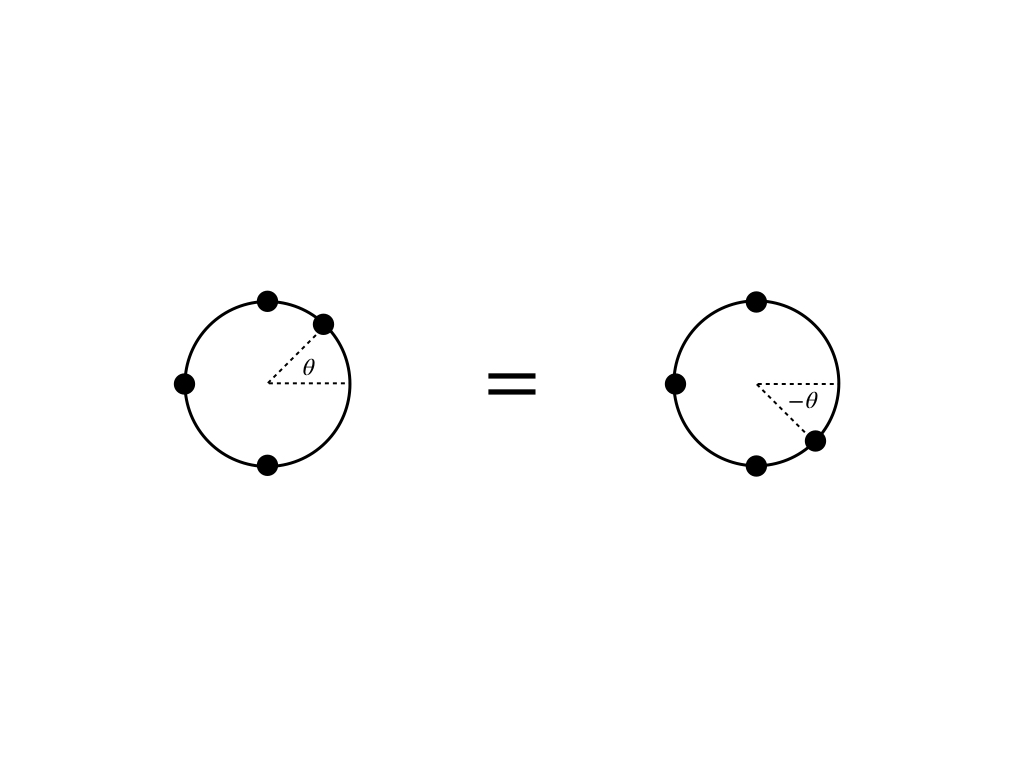
\includegraphics[width=11cm]{figures/circle}
	\caption{$\theta \to -\theta$という対称性は
		$\chi > 1$において$\chi \to \frac{\chi}{\chi - 1}$と対応する。}
\end{figure}

これは$\chi > 1$では$\mathcal{F}(\chi) = \mathcal{F}(\frac{\chi}{\chi - 1})$が成り立つ
事を意味する。
この変換は$1 < \chi < 2$の区間を$2 < \chi < \infty$へと写す事に注意すると、
$\mathcal{F}(\chi)$を決定するには$0 < \chi < 2$という区間で十分である事に気付く。
また$\chi = 2$は固定点なので、$\mathcal{F}$の一階微分の$\chi = 2$における値は0であるという条件もつく。

$\mathcal{F}_{n+1}$と$\mathcal{F}_n$の間の関係式
\eqref{eq:F_n+1_and_F_n}式を$\chi$を用いて書き直すと
\begin{align}
	\mathcal{F}_{n+1}(\chi)
	= \int_0^2 \frac{d\tilde{\chi}}{\tilde{\chi}^2}\ 
		K_c(\chi; \tilde{\chi})\mathcal{F}_n(\chi)
	\label{eq:F_n+1_and_F_n_in_chi}
\end{align}
となる。
$K_c(\chi; \tilde{\chi})$は次式で与えられる:
\begin{align}
	K_c(\chi; \tilde{\chi}) = \frac{1}{\alpha_0}\left[
		\frac{\chi^{2\Delta}\tilde{\chi}^{2\Delta}}{|\chi - \tilde{\chi}|^{2\Delta}}
		m(\chi, \tilde{\chi}) + \sgn(\tilde{\chi} - 1)
		\frac{\chi^{2\Delta}\tilde{\chi}^{2\Delta}}
			 {|\chi + \tilde{\chi} - \chi\tilde{\chi}|^{2\Delta}}
		m\left(\chi, \frac{\tilde{\chi}}{\tilde{\chi} - 1}\right)
	\right].
\end{align}
ここで$m(\chi, \tilde{\chi})$は次のような超幾何関数${}_2F_1$で与えられる
$\chi$と$\tilde{\chi}$に関して対称な関数である:
\begin{align}
	z \equiv \frac{1 - \min(\chi, \tilde{\chi})}{|\chi - \tilde{\chi}|},\hspace{20pt}
	B_h(x) = \frac{\Gamma(h)^2}{\Gamma(2h)}x^h\ {}_2F_1(h, h, 2h, x)
\end{align}
という2つの記号を導入して、
\begin{align}
	m(\chi, \tilde{\chi})
	= \frac{2\pi}{\sin 2\pi\Delta}{}_2F_1(1 - 2\Delta, 2\Delta, 1, z)
	- B_{2\Delta}\left(\frac{1}{1 - z}\right)
	- B_{1 - 2\Delta}\left(\frac{1}{1 - z}\right)
	\hspace{20pt} z \leq 0,
\end{align}
\begin{align}
	m(\chi, \tilde{\chi})
	= -\frac{2\pi}{z^{2\Delta}\sin 2\pi\Delta}{}_2F_1\left(
		2\Delta, 2\Delta, 1, \frac{z - 1}{z}\right)
	+ \frac{2\pi}{\sin 2\pi\Delta}{}_2F_1(2\Delta, 1 - 2\Delta, 1, z)
	\hspace{20pt} 0 \leq z \leq 1,
\end{align}
\begin{align}
	m(\chi, \tilde{\chi})
	= -\frac{2\pi}{\sin 2\pi\Delta}{}_2F_1(2\Delta, 1 - 2\Delta, 1, 1 - z)
	- B_{2\Delta}\left(\frac{1}{z}\right)
	- B_{1 - 2\Delta}\left(\frac{1}{z}\right)
	\hspace{20pt} 1 \leq z 
\end{align}
である。

\subsubsection{カシミール演算子$C_{1+2}の固有関数$}

次にカシミール演算子$C_{1+2}$の固有関数を求める。
\eqref{eq:casimir_operator}式から、$C_{1+2}$は
\begin{align}
	C_{1+2}\frac{1}{|t_{12}|^{2\Delta}}f(\chi)
	= \frac{1}{|t_{12}|^{2\Delta}}\mathcal{C}f(\chi),\hspace{20pt}
	\mathcal{C} = \chi^2(1 - \chi)\partial_{\chi}^2 - \chi^2\partial_{\chi}
\end{align}
を満たす。
$\mathcal{C}$の固有値を$h(h-1)$とすると、固有値方程式は$\mathcal{C}f = h(h-1)f$である。
この一般解は超幾何関数${}_2F_1$を用いて
\begin{align}
	\chi^h{}_2F_1(h, h, 2h, \chi),\hspace{30pt}
	x^{1-h}{}_2F_1(1-h, 1-h, 2-2h, \chi)
	\label{eq:eigenfunctions_of_C}
\end{align}
という2つの解の線型結合となる。
それで張られる空間は$f'(2) = 0$となるような関数の空間である。
またこの関数空間の内積は\eqref{eq:F_n+1_and_F_n_in_chi}式より
\begin{align}
	\innerprod{g}{f} = \int_0^2 \frac{d\chi}{\chi^2}g^*(\chi)f(\chi)
	\label{eq:innerproduct}
\end{align}
のように与えられる。規格化はこの内積から計算される。
$\mathcal{C}$がエルミート演算子であるための条件は
\begin{align}
	0
	= \innerprod{g}{\mathcal{C}f} - \innerprod{\mathcal{C}g}{f}
	= \int_0^2 d\chi\ \frac{d}{d\chi}\left[
		g^*(\chi)(1 - \chi)\frac{d}{d\chi}f(\chi)
		- \frac{d}{d\chi}g^*(\chi)(1 - \chi)f(\chi)
	\right]
\end{align}
である。
$\chi = 2$では$f$や$g^*$の一階微分が0になる事から表面項は消える。
また$\chi = 0$においても$f$や$g^*$は$\chi^{1/2}$よりも速く0となるという条件を課す事で消滅する。
加えて\eqref{eq:eigenfunctions_of_C}式の固有関数は$\chi = 1$にて対数発散が存在するため、
もう1つの条件を課す必要がある。
即ち、特異点を打ち消すためには
\begin{align}
	f &\approx A + B\log(1 - \chi)\hspace{20pt}\mathrm{for\ \ }\chi \to 1^-,\nonumber\\
	f &\approx A + B\log(\chi - 1)\hspace{20pt}\mathrm{for\ \ }\chi \to 1^+\nonumber
\end{align}
のように定数項と対数の項が1に近づくにつれ一致していなければならない。

以上を踏まえて、カシミール演算子$C_{1+2}$の固有関数$\Psi_h(\chi)$は次のように書き下す事ができる。
まず$1 < \chi$の時は
\begin{align}
	\Psi_h(\chi)
	= \frac{\Gamma\left(\frac{1}{2} - \frac{h}{2}\right)\Gamma\left(\frac{h}{2}\right)}
		{\sqrt{\pi}}
	{}_2F_1\left(\frac{h}{2},\frac{1}{2} - \frac{h}{2},\frac{1}{2},
	\frac{(2 - \chi)^2}{\chi^2}\right)
	\hspace{20pt}\mathrm{for\ \ }1 < \chi
	\label{eq:Psi_h_for_chi>1}
\end{align}
である。
また$\chi < 1$の時は
\begin{align}
	\Psi_h(\chi)
	= A\frac{\Gamma(h)^2}{\Gamma(2h)}\chi^h\ {}_2F_1(h, h, 2h, \chi)
	+ B\frac{\Gamma(1-h)^2}{\Gamma(2 - 2h)}\chi^{1-h}\ {}_2F_1(1-h, 1-h, 2-2h, \chi)
	\hspace{20pt}\mathrm{for\ \ }\chi < 1
	\label{eq:Psi_h_for_chi<1}
\end{align}
である。ここで$A$と$B$は
\begin{align}
	A = \frac{1}{\tan\frac{\pi h}{2}}\frac{\tan\pi h}{2},\hspace{20pt}
	B = A(1 - h) = -\tan\frac{\pi h}{2}\frac{\tan\pi h}{2}
\end{align}
で与えられる。
$\chi > 1$と$\chi < 1$の両方の場合において$\Psi_h = \Psi_{1-h}$という性質を持つ。
最後に$\chi \to 0$で$\Psi_h$は$\chi^{1/2}$と同じかそれ以上に速く0に近づくという条件から、
$h$について次の2つの解が存在する:
1つ目は$h = \frac{1}{2} + is$というものである。
この時$\Psi_h(\chi)$は$1 < \chi$で単調関数であり、また$1 > \chi$で振動する(非常に多く振動する)。
2つ目は$h = 2n, n \in \mathbb{N}$であり、定数$B$は消滅する。この解もまた
$0 < 1 < \chi$で単調関数であり、$1 > \chi$で振動する(0を$n$回横切る)。

\subsubsection{$K_c$の固有値}
$C_{1+2}$の固有関数$\Psi_h$に縮退はないため、$K_c$と$C_{1+2}$が可換である事から$\Psi_h$は
$K_c$の固有関数でもある。
原理的には\eqref{eq:eigen_eq_of_Kc}式から固有値$k_c(h)$を計算できるが、
ここではもっと単純な方法を取る。
固有値$h(h-1)$を持つ$C_{1+2}$の固有関数は2つのフェルミオンの共形3点関数の形を持つ:
\begin{align}
	\frac{\sgn(t_{12})}{|t_{10}|^h|t_{20}|^h|t_{12}|^{2\Delta - h}}.
\end{align}
これは任意の$t_0$や$h$において$K_c$の固有関数である。
$SL(2, \mathbb{R})$を用いて$t_0$を動かす事が可能なため、固有値$k_c(h)$は$h$にのみ依存する。
特に$t_0$を無限大に持っていけば、固有値は\eqref{eq:confomarl_K}式より
\begin{align}
	k_c(h)
	= \int dt_1 dt_2\ K_c(1, 0; t_1, t_2)\frac{\sgn(t_{12})}{|t_{12}|^{2\Delta - h}}
	= -\frac{1}{\alpha_0}\int dt_1dt_2\ 
	\frac{\sgn(1 - t_1)\sgn(-t_2)\sgn(t_{12})}
	{|1-t_1|^{2\Delta}|t_2|^{2\Delta}|t_{12}|^{2-2\Delta-h}}
\end{align}
となる。
この積分の実行には
\begin{align}
	\frac{\sgn(t)}{|t|^a} = \int\frac{\d\omega}{2\pi}
		e^{-i\omega t}c(a)|\omega|^{a-1}\sgn(\omega),\hspace{20pt}
		c(a) = 2i2^{-a}\sqrt{\pi}
		\frac{\Gamma\left(1-\frac{a}{2}\right)}{\Gamma\left(\frac{1}{2}+\frac{a}{2}\right)}
\end{align}
を用いると良い。
結果は
\begin{align}
	k_c(h) = \frac{1}{\alpha_0}\frac{c(2-2\Delta-h)}{c(2\Delta-h)}c(2\Delta)^2
	\label{eq:eigenvalue_of_Kc}
\end{align}
となる。
$k_c(h)$は全ての$h = \frac{1}{2} + is$や$h = 2n$で実数となる。
特に連続的なスペクトラムに対しては負、離散的なスペクトラムだと正となる。
$q = 4, \infty, 2$の場合について具体的な式は
\begin{align}
	k_c(h) &= -\frac{3}{2}\frac{\tan\frac{\pi(h - 1/2)}{2}}{h - \frac{1}{2}}
	\hspace{30pt}q = 4,\\
	k_c(h) &= \frac{2}{h(h-1)}
	\hspace{61pt}q = \infty,\\
	k_c(h) &= -1
	\hspace{87pt}q = 2
\end{align}
となる。特に$q = 4, \infty$の時$k_c(h=2) = 1$となり、\eqref{eq:geometric_series_of_F}
の級数が発散する。
この$h = 2$についての正しい取り扱いは後に議論する。

\subsubsection{$\innerprod{\Psi_h}{\Psi_h}$と$\innerprod{\Psi_h}{\mathcal{F}_0}$}

次に\eqref{eq:final_F_chi}式の計算に必要な2つの内積
$\innerprod{\Psi_h}{\Psi_h}$と$\innerprod{\Psi_h}{\mathcal{F}_0}$を求める。
連続的なスペクトラム$h = \frac{1}{2} + is$に関しては
\begin{align}
	\innerprod{\Psi_h}{\Psi_h} = \frac{\pi\tan\pi h}{4h-2}2\pi\delta(s - s')
\end{align}
で与えられ、また離散的なスペクトラム$h = 2n, n\in\mathbb{N}$に関しては
\begin{align}
	\innerprod{\Psi_h}{\Psi_h} = \frac{\delta_{hh'}\pi^2}{4h-2}
\end{align}
となる。

$\chi$の関数としての$\mathcal{F}_0$は
\begin{align}
	\mathcal{F}_0(\chi) = \left\{
	\begin{array}{l}
		-\chi^{2\Delta} + \left(\frac{\chi}{1 - \chi}\right)^{2\Delta}
		\hspace{20pt}0 < \chi < 1,\\
		-\chi^{2\Delta} - \left(\frac{\chi}{\chi - 1}\right)^{2\Delta}
		\hspace{20pt}1 < \chi < \infty
	\end{array}\right.
\end{align}
で与えられる。
以下では内積$\innerprod{\Psi_h}{\mathcal{F}_0}$の計算には連続的なスペクトラムについてのみ考える。
離散的なスペクトラムの場合は$h$について解析接続する事で得られる。
固有関数$\Psi_h$は連続スペクトラムにおいて次のような積分表示を持つ:
\begin{align}
	\Psi_h(\chi) = \frac{1}{2}\int_{-\infty}^{\infty}dy\ 
	\frac{|\chi|^h}{|y|^h|\chi - y|^h|1 - y|^{1-h}}.
\end{align}
この積分表示を用いて$\innerprod{\Psi_h}{\mathcal{F}_0}$の積分を行う。
$\chi\to\frac{\chi}{\chi-1}$の変換で$\Psi_h(\chi) = \Psi_h\left(\frac{\chi}{\chi-1}\right)$
であるが、$\mathcal{F}_0$はこの変換で、$\chi > 1$の時は対称、$\chi < 1$の時は反対称となる。
この性質を用いると
\begin{align}
	\innerprod{\Psi_h}{\mathcal{F}_0}
	= -\frac{1}{2}\int_{-\infty}^{\infty}dyd\chi\ 
	\frac{\sgn(\chi)}{|\chi|^{2-h-2\Delta}|\chi-y|^h|1-y|^{1-h}|y|^h}
\end{align}
を得る。
この積分は、積分領域を分割し、それぞれの領域でオイラーの$\beta$関数を用いると実行できる。
便利な表式として
\begin{align}
	\innerprod{\Psi_h}{\mathcal{F}_0} = \frac{\alpha_0}{2}k_c(h)
\end{align}
というものがある。

\subsubsection{全ラダーダイアグラムの総和}
ここまでの議論を踏まえて、4点関数は
\begin{align}
	\mathcal{F}(\chi)
	&= \sum_h\Psi_h(\chi)\frac{1}{1 - k_c(h)}
		\frac{\innerprod{\Psi_h}{\mathcal{F}_0}}{\innerprod{\Psi_h}{\Psi_h}}\nonumber\\
	&= \alpha_0\int_0^{\infty}\frac{ds}{2\pi}\frac{2h-1}{\pi\tan\pi h}
		\frac{k_c(h)}{1-k_c(h)}\Psi_h(\chi)
	+ \alpha_0\sum_{n=1}^{\infty}\left[
		\frac{2h-1}{\pi^2}\frac{k_c(h)}{1-k_c(h)}\Psi_h(\chi)
	\right]_{h=2n}
	\label{eq:all_sum_of_ladders}
\end{align}
となる。
ここで1つの問題が生じる: $n = 1$の項は$k_c(2) = 1$より発散する。
これを取り扱うには共形極限から少しずれた領域に行かなければならない。
ここでは、ひとまず$h\neq2$となる固有関数のみを扱い、その寄与を$\mathcal{F}_{h\neq2}$とする.
この時
\begin{align}
	\frac{2}{\tan\pi h} = \frac{1}{\tan\frac{\pi h}{2}} - \frac{1}{\tan\frac{\pi(1-h)}{2}}
\end{align}
という公式を使い、$s$の積分領域を実数全体$-\infty\to\infty$に広げ、
被積分関数が持つ$h\to1-h$の下での反対称性を用いて複数ある項を1つに直すと
\begin{align}
	\frac{\mathcal{F}_{h\neq2}}{\alpha_0}
	= \int_{-\infty}^{\infty}\frac{ds}{2\pi}\frac{h - 1/2}{\pi\tan(\pi h / 2)}
		\frac{k_c(h)}{1-k_c(h)}\Psi_h(\chi)
	+ \sum_{n=2}^{\infty}\mathrm{Res}\left[
			\frac{h-1/2}{\pi\tan(\pi h/2)}\frac{k_c(h)}{1-k_c(h)}\Psi_h(\chi)
		\right]_{h=2n}.
\end{align}
となる。
級数の項は$\frac{1}{\tan(\pi h/2)}$の極の留数を走る総和として書いた。
第1項目の被積分関数と第2項目の級数の中身が同じであるため、
右辺全体を複素$h$平面のある曲線$\mathcal{C}$上の線積分として理解できる:
\begin{align}
	\frac{1}{2\pi i}\int_{\mathcal{C}}dh
	= \int_{-\infty}^{\infty}\frac{ds}{2\pi}
	+ \sum_{n=1}^{\infty}\mathrm{Res}_{h=2n}.
\end{align}
ここで、$\Psi_h$は$h = 1 + 2n$に極を持つが、これは$1/\tan(\pi h / 2) = \pm 1/\infty$によって
相殺される。従って全体では$h = 2n$のみに極を持つ。

$\Psi_h$が$\chi > 1$の場合\eqref{eq:Psi_h_for_chi>1}式と
$\chi < 1$の場合$\eqref{eq:Psi_h_for_chi<1}$式で違うため、この2つのケースで場合分けして考える。
まず$\chi > 1$の時、曲線$\mathcal{C}$を$s$軸から無限遠へ右にずらす事ができる。
これによって$h = 2n$における極の総和はキャンセルされるが、
$k_c(h) = 1$となる$h = h_m$における極を選ぶ事となり、
\begin{align}
	\mathcal{F}_{h\neq 2}(\chi)
	= -\alpha_0\sum_{m=0}^{\infty}\mathrm{Res}\left[
		\frac{h - 1/2}{\pi\tan(\pi h / 2)}\frac{k_c(h)}{1 - k_c(h)}\Psi_h(\chi)
	\right]_{h=h_m}
	\hspace{30pt}\chi > 1
\end{align}
を得る(図\ref{fig:poles})。
\begin{figure}[ht]
	\centering
	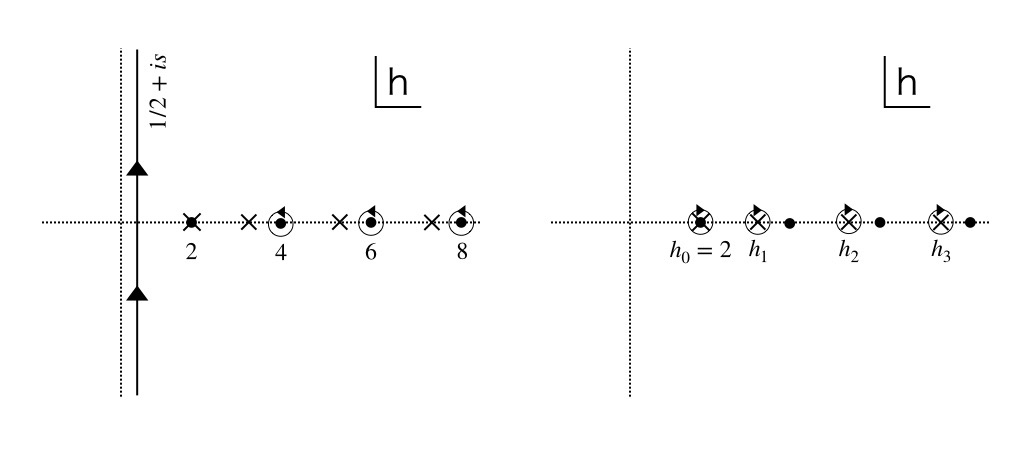
\includegraphics[width=11cm]{figures/poles}
	\caption{$h$平面における極。$h = 2n$における極を点、$k_c(h) = 1$となるような
	$h = h_m$における極をバツ印で表した。$h = 2 = h_0$では極が重なるため点とバツ印を重ねている。
	$h$の連続スペクトラム$h = 1/2 + is$の直線は
	右へずらす事ができ、点で表した$1/\tan(\pi h/2)$の極を相殺し、バツ印の極を選ぶ事になる。}
	\label{fig:poles}
\end{figure}

次に$\chi < 1$の場合について考える。
この場合は\eqref{eq:Psi_h_for_chi<1}式の${}_2F_1(1-h,1-h,2-2h,\chi)$を大きい$h > 0$に
持っていく事ができないため、少し回り道をする必要がある。
最初に、被積分関数の中の$\tan(\pi h/2)$を$\tan(\pi h)$に置き換えるために、
${}_2F_1$以外の残りの部分が持つ$h\to 1-h$の下での反対称性を利用する。
これによって$h\to 1-h$の下で対称となる被積分関数を得る。
この対称性を使って\eqref{eq:Psi_h_for_chi<1}式の$B$を$A$に置き換えれば、
\begin{align}
	\frac{\mathcal{F}_{h\neq 2}(\chi)}{\alpha_0}
	= \int &\frac{ds}{2\pi}\frac{h-1/2}{\pi\tan(\pi h/2)}
		\frac{k_c(h)}{1-k_c(h)}\frac{\Gamma(h)^2}{\Gamma(2h)}
		\chi^h\ {}_2F_1(h, h, 2h, \chi)\nonumber\\
	&+ \sum_{n=2}^{\infty}\mathrm{Res}\left[
		\frac{h-1/2}{\pi\tan(\pi h/2)}\frac{k_c(h)}{1-k_c(h)}\frac{\Gamma(h)^2}{\Gamma(2h)}
		\chi^h\ {}_2F_1(h, h, 2h, \chi)
	\right]_{h=2n}
\end{align}
という式に至る。
ここで留数の総和において、$h$が偶数の時
$\Psi_h(\chi) = \frac{\Gamma(h)^2}{\Gamma(2h)}\chi^h\ {}_2F_1(h, h, 2h, \chi)$
となる事を用いた。
この被積分関数は$\chi > 1$の場合のように右へずらす事が可能であり、選ぶべき留数が$k_c(h)=1$
となる$h = h_m$におけるものとなり、最終的に
\begin{align}
	\mathcal{F}_{h\neq 2} = -\alpha_0\sum_{m=0}^{\infty}\mathrm{Res}\left[
		\frac{h-1/2}{\pi\tan(\pi h/2)}\frac{k_c(h)}{1-k_c(h)}\frac{\Gamma(h)^2}{\Gamma(2h)}
		\chi^h\ {}_2F_1(h, h, 2h, \chi)
	\right]_{h=h_m}
	\hspace{30pt}\chi < 1
\end{align}
を得る。

\subsection{$h = 2$の場合の取り扱い}
$K_c$は固有値$k_c(h) = 1$を持つため、\eqref{eq:geometric_series_of_F}式の級数が発散する。
$k_c(h) = 1$となるのは$h = 2$における$SL(2, \mathbb{R})$のカシミール演算子$C_{1+2}$の固有関数である。
4点関数の有限な解を得るために、$K$を摂動的に共形極限から$\delta K$だけずらした場所でその固有関数を
扱う必要がある。
摂動による補正$\delta K$は、$K$を構成する2点関数$G$の非共形極限におけるリーディングオーダーでの補正
$\delta G$から生じる。
摂動パラメータは結合の大きさの逆数$(\beta J)^{-1}$である。

共形極限において、零温度と有限温度での両方の解$\eqref{eq:conformal_ansatz}$式は
$t$のパラメータ付け替え不変性によって互いに等しいものであったが、摂動$\delta K$によって
共形対称性が破れるため、2つの解を等しいとする事はできない。
そこで最初から有限温度で議論し、周期を$\beta$から$2\pi$にするために
角度座標$\theta = 2\pi t / \beta$を導入する。値の範囲は$\theta \in [0, 2\pi]$である。
これは$\beta = 2\pi$と設定して議論を始めようとしているとも言える。
$\theta$は周期的ユークリッド時間である。

また$K$を直接論じるよりも、それを対称化した$\tilde{K}$の方が話を進めやすい。
\eqref{eq:symmetric_K}式で$t\to\theta$と変数変換すると
\begin{align}
	\tilde{K}(\theta_1, \theta_2; \theta_3, \theta_4)
	= -J^2(q-1)
		|G(\theta_{12})|^{\frac{q-2}{2}}
		G(\theta_{13})G(\theta_{24})
		|G(\theta_{34})|^{\frac{q-2}{2}}
\end{align}
となる。
またこの積分核$\tilde{K}$の反対称な固有関数を
\begin{align}
	\Psi_{h,n}^{\mathrm{exact}}(\theta_1, \theta_2)
	= - \Psi_{h,n}^{\mathrm{exact}}(\theta_2, \theta_1)
\end{align}
と書く事にする。
ここで添字$h$はあるラベルであり、後に詳しく説明する。
また$n$はフーリエ展開した際の$e^{-in(\theta_1 + \theta_2)/2}$の中の$n$である。
$\tilde{K}$は次式で与えられる内積において対称となる:
\begin{align}
	\innerprod{\Psi}{\Phi} \equiv
	\int_0^{2\pi}d\theta_1d\theta_2\ \Psi^*(\theta_1, \theta_2)\Phi(\theta_1, \theta_2).
\end{align}

4点関数の表式を得るためには、輪を持たないラダーダイアグラム$\mathcal{F}_0$が
反対称単位行列
\begin{align}
	I(\theta_1, \cdots, \theta_4)
	= -\delta(\theta_{13})\delta(\theta_{24}) + \delta(\theta_{14})\delta(\theta_{23})
	= -2\sum_{h,n}\Psi_{h,n}^{\mathrm{exact}}(\theta_1, \theta_2)
		\Psi_{h,n}^{\mathrm{exact}*}(\theta_3, \theta_4)
\end{align}
に作用する$\tilde{K}$に比例するという事を用いると良い。
おおよそ$\mathcal{F} = (1 - \tilde{K})^{-1}\tilde{K}\cdot I$の様に書き表す事ができ、
より正確には
\begin{align}
	\left[(q-1)J^2G(\theta_{12})^{\frac{q-2}{2}}G(\theta_{34})^{\frac{q-2}{2}}\right]
	\mathcal{F}(\theta_1,\cdots,\theta_2) = 
	2\sum_{h,n}\frac{k(h,n)}{1-k(h,n)}
		\Psi_{h,n}^{\mathrm{exact}}(\theta_1, \theta_2)
		\Psi_{h,n}^{\mathrm{exact}*}(\theta_3, \theta_4)
	\label{eq:fourpointfunc_in_theta}
\end{align}
となる。ここで$k(h,n)$は
固有関数$\Psi_{h,n}^{\mathrm{exact}}(\theta_1, \theta_2)$に対応する固有値である。
適切な固有関数の完全系の下で、この4点関数の表式はあらゆるカップリングの大きさ$\beta J$において正しい。

共形極限$\beta J \gg 1$に行くと、前節までの議論と接続できる。
固有関数$\Psi_{h,n}^{\mathrm{exact}}$は、
$SL(2,\mathbb{R})$に属する固有値$h(h-1)$を持つカシミール演算子$C_{1+2}$の固有関数$\Psi_{h,n}$となり、
固有関数も$k(h,n)\to k_c(h)$の様に$h$だけの関数になる。
また\eqref{eq:fourpointfunc_in_theta}式の$n$を走る総和は
($t$を$t = \tan\frac{\theta}{2}$によって円周上に射影した後で)
$\mathcal{F}_{h\neq 2}$の$\Psi_h$が現れる表式を与える。

4点関数の計算において$h = 2$からは無限大の寄与を得てしまう。
これはフーリエインデックス$n$について走る関数族$\Psi_{2,n}$によって与えられる。
この無限大を対処するには、共形極限から少し離れて共形対称性を破った上で
リーディングオーダーでの補正を求める必要がある。
特に共形極限での固有値$k_c(h)$への補正を計算する:
\begin{align}
	k(2, n) = 1 - O\left(\frac{1}{\beta J}\right).
\end{align}

\subsubsection{$\Psi_{2,n}$とパラメータ付け替え}
共形極限では、$\tilde{K}$は共形伝搬関数\eqref{eq:conformal_ansatz}式の有限温度における表式を用いて
\begin{align}
	\tilde{K}_c(\theta_1, \cdots, \theta_4)
	= -\alpha_0
		\frac{1}{|2\sin\frac{\theta_{12}}{2}|^{1-2\Delta}}
		\frac{\sgn(\theta_{13})}{|2\sin\frac{\theta_{24}}{2}|^{2\Delta}}
		\frac{\sgn(\theta_{24})}{|2\sin\frac{\theta_{34}}{2}|^{2\Delta}}
		\frac{1}{|2\sin\frac{\theta_{13}}{2}|^{1-2\Delta}}
\end{align}
と表される。ここで$\alpha_0$は\eqref{eq:alpha_0}式で与えられる。
この対称積分核$\tilde{K}_c$は有限温度における$SL(2, \mathbb{R})$のリー代数の各生成子と可換である:
\begin{align}
	\hat{P} = e^{-i\theta}\left(\partial_{\theta} - \frac{i}{2}\right),\hspace{30pt}
	\hat{K} = -e^{i\theta}\left(\partial_{\theta} + \frac{i}{2}\right),\hspace{30pt}
	\hat{D} = i\partial_{\theta}.
\end{align}


\pagebreak
